This section will discuss the feasibility of Artificial Neural Network as a technology for prediction of electricity prices and wind power. The hypothesis presented in Section~\ref{sec:theHypothesis} and the experimental results will be the basis for the discussions. Following quotation from the hypothesis section has been pointed out:

\begin{quotation}
\textit{Artificial Neural Networks can be characterised as Machine Learning\cite{18} and historical data that is relevant for the specific task will be used for training. The goal is to investigate and identify (through analysis and experiments) the importance of the influential factors to be included and represented in these datasets. Based on this we examine the feasibility of a Back Propagation Artificial Neural Network as a technology for predicting electricity prices and wind power.}
\end{quotation}

\noindent The hypotheses take its outset in how to utilize the Artificial Neural Network best possible by analysing the influential factors, representing them appropriately and verifying it through experiments. Answering the feasibility question regarding ANN as a proper technology for predicting electricity price and wind power will be based on these parameters. It will be structured in the following way:

\begin{itemize}
\item Input analysis and transparency: This section will be dealing with the importance of investigating the influential factors.
\item Trustworthiness: The section considers the conducted experiments to verify the analysis and how to trust them.
\item Feasibility: Will conclude on the feasibility based on \#1, \#2 and our experimental results.
\end{itemize}

\subsection{Input analysis and transparency}
Artificial Neural Networks as a technology for prediction in the electricity market is much dependent on the analysis and experiments surrounding it. The experiment discussions above highlight the need for analysing and documenting characteristics of what is to be predicted by the ANN. Machine Learning is data-driven\cite{18} and the analysis together with experiments point out the influential input parameters to include in the dataset that is the basis for the data-driven learning. The analysis will identify the input parameters to test and the experiments will either reject or verify what came out of the analysis. The result will be the best network setting along with a common understanding of exactly why these input parameters did the job for this market and why others did not. In continuation of this lies the need for transparency when using ANNs since omitting it will make it difficult to draw on the experience of others and make comparisons between systems due to the black box nature of the technology. Comparisons are of course possible if both attempted to predict the exact same market and used the exact same performance measure. 

In Section~\ref{sec:inputParameterDiscussion} we discuss the difference in experimental setups from publication to publication and how it becomes difficult to imitate when the information about it is incomplete. Based on discussions throughout the thesis and the comparison conducted in the experiment from Section~\ref{sec:priceExperimentThree} we argue that such comparisons are not even fair due to the lack of documentation regarding input analysis, dataset and experiments. An example of a meaningful price parameter in the Danish electricity market which does not apply for all markets is wind speed due to the large amount of wind mills in Denmark. This parameter shows a co-relation of 0,28 (Section~\ref{sec:Price}) and it is clear from the analysis why it has been included in the experiments where the influence is verified even to a greater extend than expected --- predicting the prices in a country without many wind mills should probably not expect the same benefits when using our setup with wind speed which should be apparent from the analysis in Section~\ref{sec:priceWeatherInfluence}. Another example exist for wind power where demand is analysed to greatly influence the production but is instead substituted with air density in the best prediction due to air density being calculated with temperature and pressure. Temperature highly influences demand and because pressure is close to constant the air density express temperature (see Section~\ref{sec:predictionBasicInputParams}). Dataset manipulation can greatly affect the predictions as well as discussed in Section \ref{sec:matrixTrimmingDiscussion}. Matrix representation of the input parameters proved to affect both datasets positively. The trimming only improved the price predictions but with a substantial improvement. If not documented properly the use of these input parameters and dataset manipulations are unclear and it would require investigation and assumptions by others to replicate. The overall benefits obtained in our experiments will most likely \emph{not} be the same when used in markets with different properties. It emphasizes what have been said earlier, namely that transparency in an analysis is necessary to make comparisons and knowledge sharing possible but at the same time to identify the best possible setting yourself. The feasibility of the ANN should not be judged on its results alone (MAE, MAPE) but also on how and why the input parameters were selected and represented in the dataset. Both because what makes it applicable in one setting does not necessarily apply for another but also because we need to trust that the dataset is selected and tested based on a satisfactory foundation --- the resulting error can best be explained by looking at exactly what conditions constituted it. For instance, all our prediction experiments use last hours production or price as input and the accuracy will drop significantly if the day-ahead forecast uses the predicted value (which is the case for this thesis because it mimics real use) instead of the ideal. This is discussed in Section~\ref{sec:stepAheadForecastingDiscussion} but the point is that this information is necessary to have any idea of the result. This leads to the trustworthiness of a system in terms of the experiments performed to verify the inputs which will be the topic of the next section.  
\todo{we could have been more structured --> trend analysis and statistics}

\subsection{Trustworthiness}
A reliable prediction must have included all the right input parameters based on a comprehensive analysis in combination with a series of experiments that validate the findings. Section~\ref{sec:unseenDataDiscussion} emphasize and discuss the necessity of simulating predictions for at least a year to strengthen results. The year contains many different days and the seasons have different conditions, e.g. winter calls for heating and a lot of indoor activity whereas the summer is equal to holiday and being outdoor which is obviously reflected in the prices seen in Section~\ref{sec:seasonality}. The changes are also apparent for wind power but mostly due to the changes in weather conditions during the year (see Section~\ref{sec:windProdSeasonality}). The wind power seasonality is shown in graphs from Section~\ref{sec:windPowerBestPredictionGraphs} where spring and fall have been highlighted in Figure~\ref{fig:bestWPPredictSpringForDiscussion} and~\ref{fig:bestPredictWPFallForDiscussion} (the difference between the two should be apparent). We have shown examples of articles predicting only individual days or weeks and argue it to be sufficient (discussed in Section~\ref{sec:inputParameterDiscussion}). We consider it necessary to simulate the predictions for an entire year in all experiments so that all conditional changes of every season are included and reflected in the results --- this is of course time-consuming but argued to be necessary. Besides from the impact of different seasons our results showed a great variation in error according to the starting point of the prediction. It emphasizes how different scenarios have different results and therefore must be covered during testing. The discussion is elaborated in Section~\ref{sec:stepAheadForecastingDiscussion} where the potential elevated error depends highly on the starting point of the prediction. The trustworthiness of the prediction is related to how thoroughly it has been tested and how many scenarios have been covered to simulate the greater part of possible use cases. 

\begin{figure}[H]
\centering
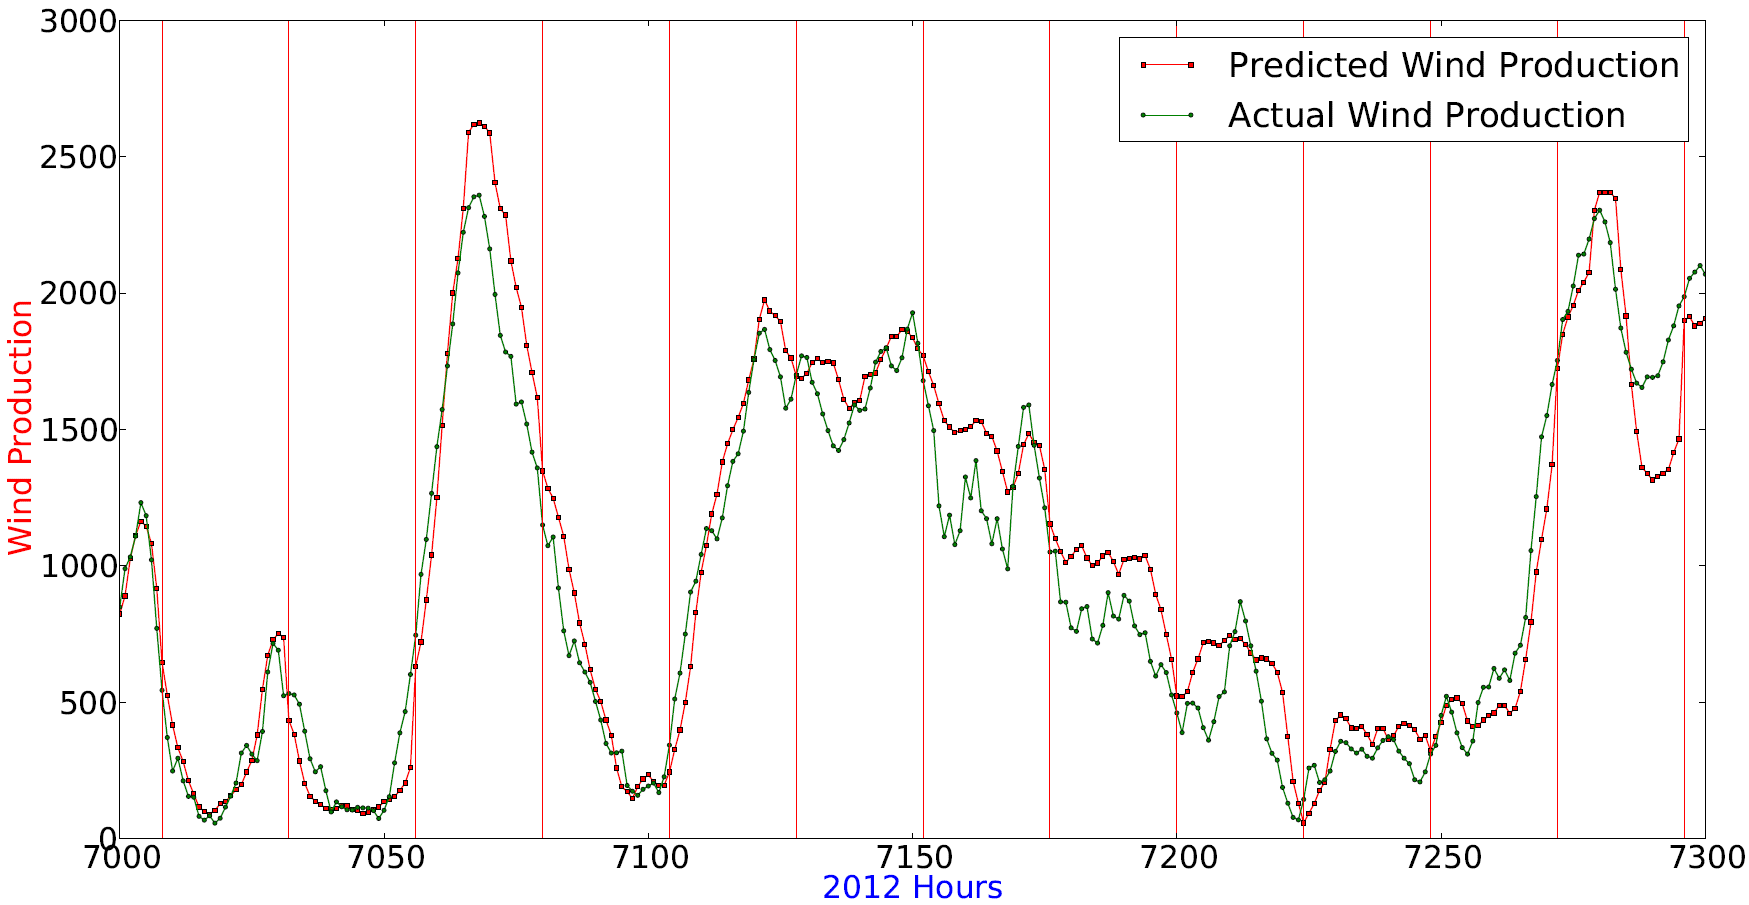
\includegraphics[width=0.99\linewidth]{billeder/bestPossiblePredictionWindProduction7000-7300_Fall.png}
\caption{Best prediction for 300 hours for Oct-Nov (Fall)}
\label{fig:bestPredictWPFallForDiscussion}
\end{figure}

\begin{figure}[H]
\centering
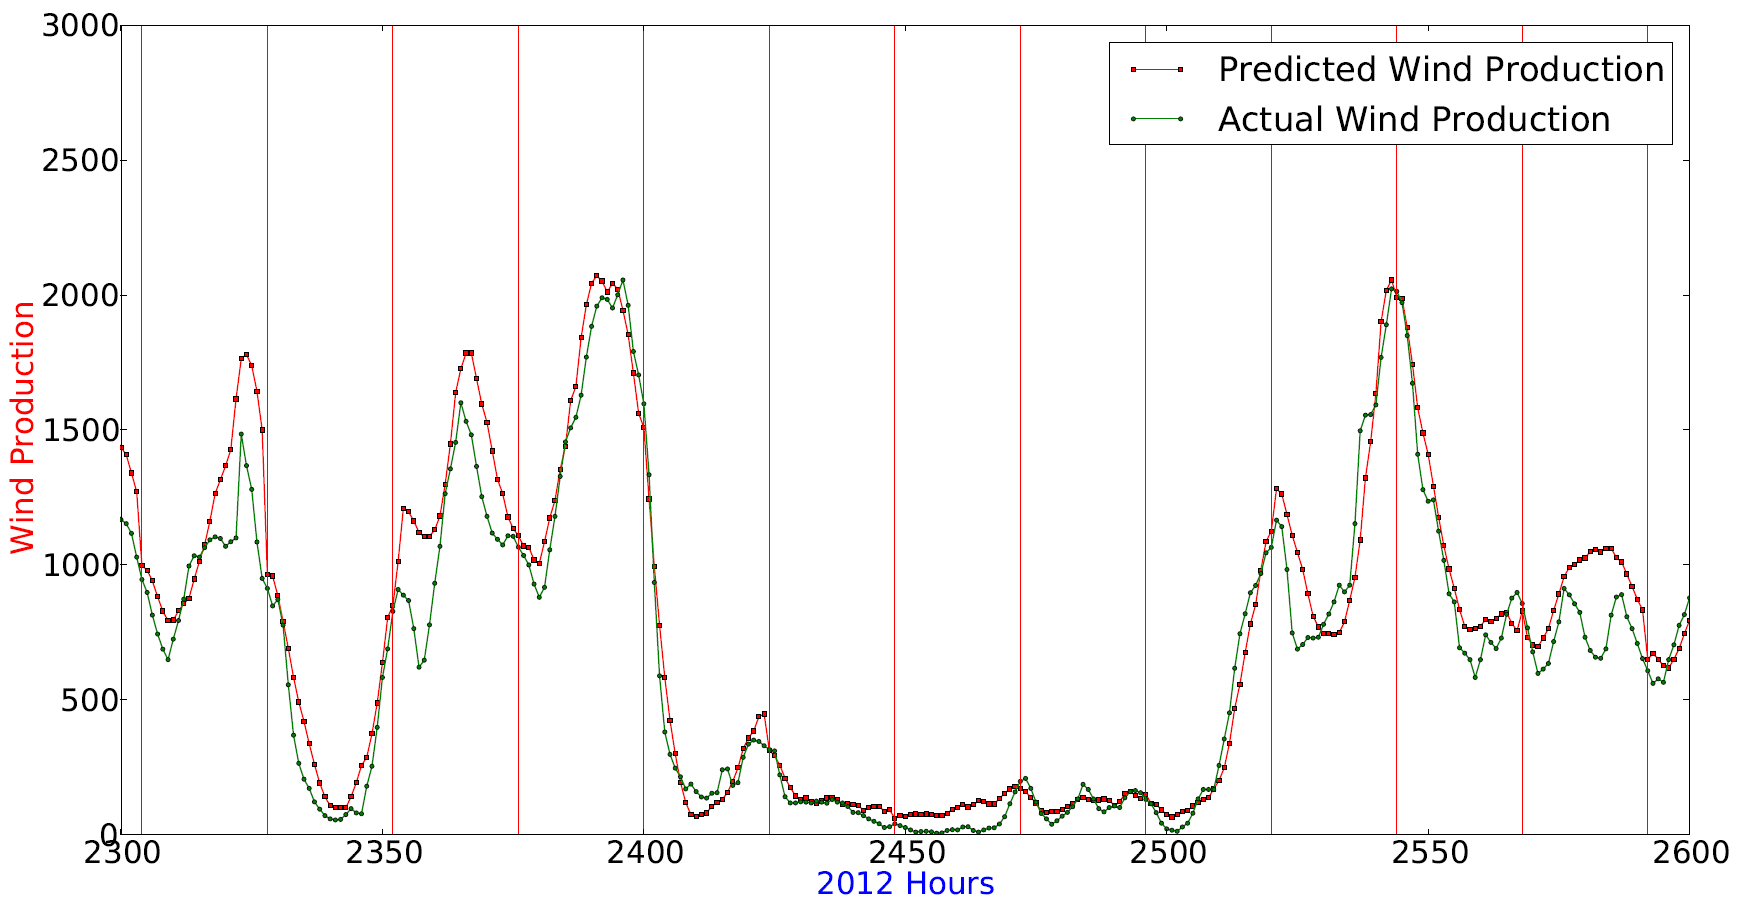
\includegraphics[width=0.99\linewidth]{billeder/bestPossiblePredictionWindProduction2300-2600_April_Spring.png}
\caption{Best prediction for 300 hours of April (Spring)}
\label{fig:bestWPPredictSpringForDiscussion}
\end{figure}

When arguing the need for testing on an entire year we must highlight the different results when running the same prediction again (discussed in detail in Section~\ref{sec:unseenDataDiscussion}). In our thesis we use an entire year to cover all conditions during a year as well as predicting similar days more than once. An alternative could be to run the yearly experiments more than once and deliver the average error for all test runs. This would strengthen the results but must be a trade-off between time constraints and trying to cover most cases (exemplified in Section~\ref{sec:windPowerBestPredictionGraphs}). Another impact from our dataset could be the fact that our testing set does not contain any predicted values. This can negatively affect the predictions when used in a real life setting and testing of this must be included in future work. We still consider the actual values to be sufficient since they look exactly the same and can simulate the predicted values in our experiments (simulation of a real setting). Furthermore, it gives us the opportunity to simulate all possible predictions of an entire year (since historical prediction data is not available to our knowledge) which our experiments show the importance of as described above. The analysis of the actual values show what influence the electricity price and wind power and in future work we must rely on other professionals to give us the best possible predictions of consumption and weather so that they are accurate enough to be consistent with the analysis. The weather predictions will deviate from the analysis \emph{only} if they are inconsistent and inaccurate but as described in Section~\ref{sec:dataCollection} the accuracy of 24 hours weather prediction is 97\%. We consider the results obtained in this thesis valid because the potential decrease in accuracy would apply for all results, highly ranked or not. It correctly shows the co-relation between input/output, the ranking of results and the input combinations used. It must be pointed out that the results are not definitive but gives a clear indication of the influences of wind power and electricity prices as well as showing what data manipulations work for the Danish electricity market. The transparency of an Artificial Neural Network and its black box is considered a key to the feasibility of the predictions themselves because it implies trustworthiness. Transparency becomes of even greater importance when applying the ANN in a real setting for decision making --- will be discussed next.

\subsection{Feasibility}
The feasibility of the Artificial Neural Networks as a proper technology for prediction will be based on conclusions from the discussions just above and the experimental results. Results will not be compared to other Artificial Neural Networks since it has been found out of scope and even unfair. Early discussions showed how comparisons between ANNs require rebuilding and imitation of the experimental setups and then running it on our own datasets. This can be very difficult and even meaningless due to different market conditions and incomplete analysis and documentation. We made an example by attempting it in Section~\ref{sec:priceExperimentThree} where our own approach obtained 11\% better MAE than the other on our dataset. Without any prober analysis of their market, dataset and experimental setup we have no foundation for making any assumptions of their resulting error. We can conclude that with the information we were able to extract it did not work for the Danish electricity market. Section~\ref{sec:influenceOfTrendInCalcInput} presents a publication that forecasts electricity spot prices for Western Denmark (DK-1) from Nord Pool Spot. Their results have been used to position our approach and determine the feasibility of our experimental results. We achieved 34 DKK better MAE than the simplest approach, 2 and 4 DKK worse than their ARIMA and Holt-Winters approach and 11 DKK worse than their best approach. The results are not definitive but can be used as an indicator for the Artificial Neural Networks ability to predict electricity prices for western Denmark. Furthermore they present the Wavelet Neural Network as a technology that most likely can obtain similar results to their best approach which could be explored further in future work.

The feasibility of the proposed ANN can be seen as a direct result of the identified input parameters and their representation. The analysis, the actual selection of inputs and the experiments is what constitutes the prediction and explains the obtained experimental results --- it is also what creates trustworthiness in the results (MAE, MAPE). The prediction is data-driven and as a result no better than the dataset it is trained upon. The feasibility should therefore be mentioned based on the analysis of input parameters and how they were validated through experiments. This of course presupposes that the prediction experiments must cover as many scenarios as possible. Days are different and the overall feasibility of the ANN is not conveyed if not tested on a satisfactory amount of data. We argue that the final prediction error cannot stand alone without a description of exactly what constituted it and why. We have in this thesis satisfied the above by a thorough analysis of the influential factors for electricity price and wind power for Western Denmark in Chapter~\ref{ch:theANNs} which have been validated through various experiments performed on an entire year in Chapter~\ref{ch:experimentalResults}. The experimental results show how the predictions evolve from experiment to experiment and how the different strategies affect the prediction results which is in agreement with our original purpose, i.e. to investigate and identify the importance of influential factors to be included and represented in the dataset. The best result for wind power misses its target by 121,02 MWh out of the interval from 0-2753 which corresponds to 4,4\% of the 2753 possible values. The influential factors was wind speed, temperature, last known wind power, time of day and historical volatility. The best electricity price prediction achieved 45,11 DKK out the interval of 61-632 which corresponds to 7,9\% out of 571 values (632-61) on demand, wind speed, temperature, time of day, time of week, season of year, skewness and historical volatility. Examples of the predictions can be seen for wind power in Figure~\ref{fig:abilityToPredictWindPower} and for the electricity price in Figure~\ref{fig:abilityToPredictElectricityPrice} --- the graphs are taken from Section~\ref{sec:windPowerBestPredictionGraphs} and ~\ref{sec:priceExperimentFour}. The most striking thing from the graphs is the difference in volatility which makes the electricity price harder to predict (which has also been stated throughout the analysis and experiments).

\begin{figure}[H]
\centering
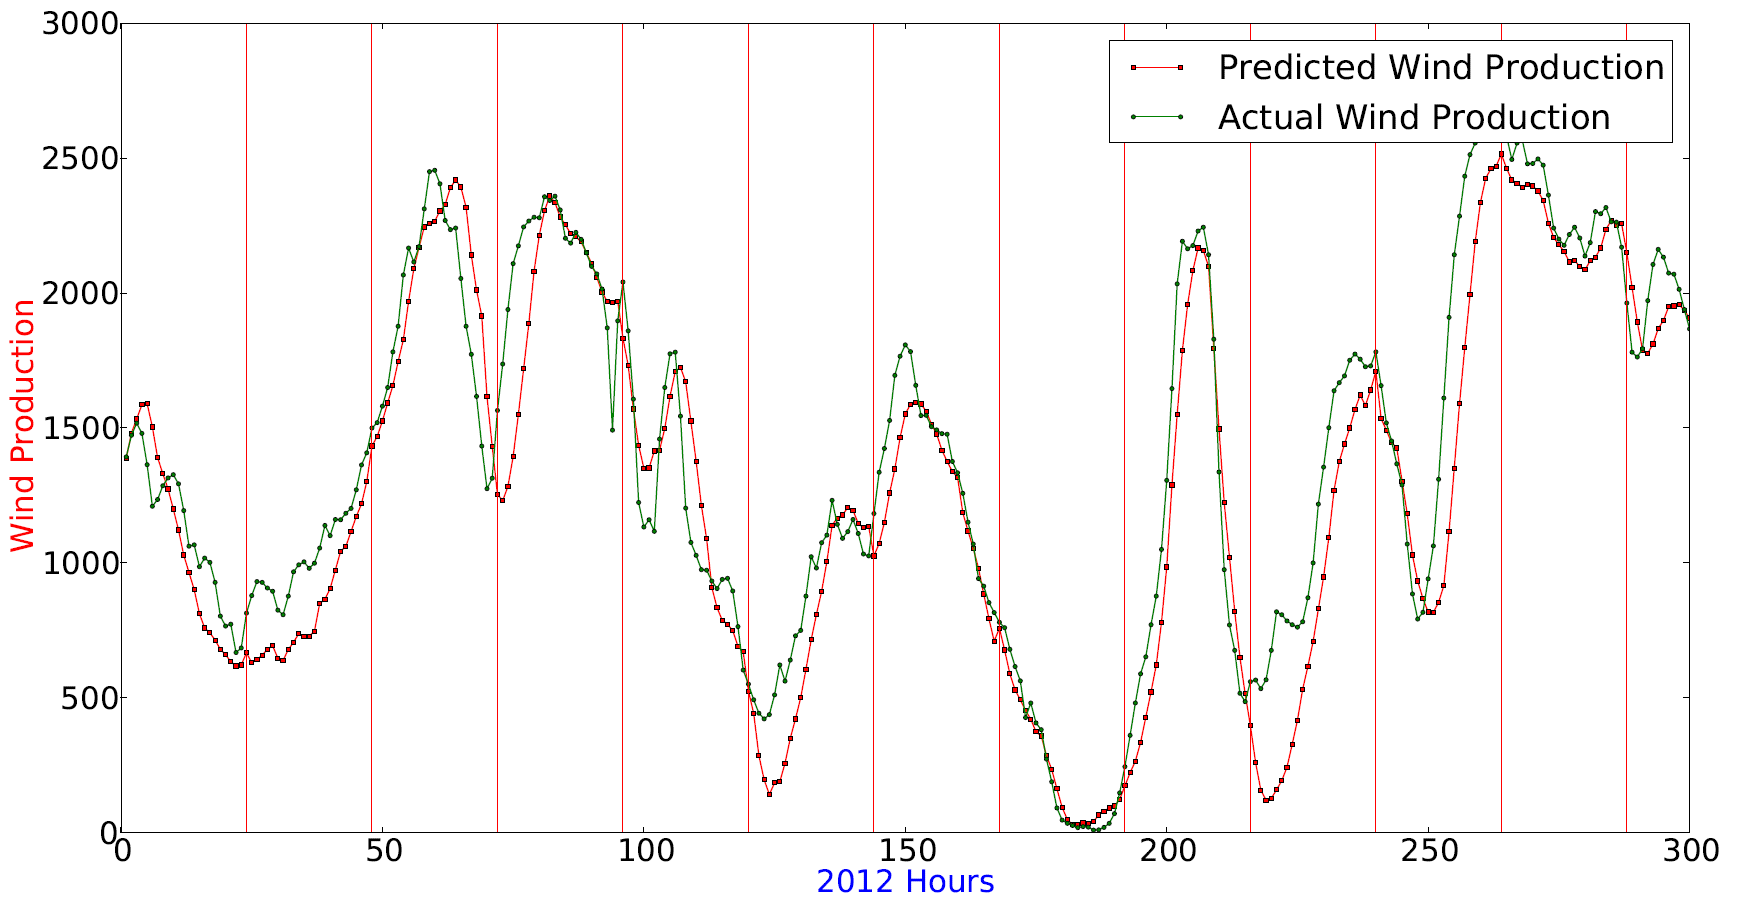
\includegraphics[width=0.99\linewidth]{billeder/bestPossiblePredictionWindProduction0-300.png}
\caption{Wind Power best prediction for 300 hours of January (Winter)}
\label{fig:abilityToPredictWindPower}
\end{figure}

\begin{figure}[H]
\centering
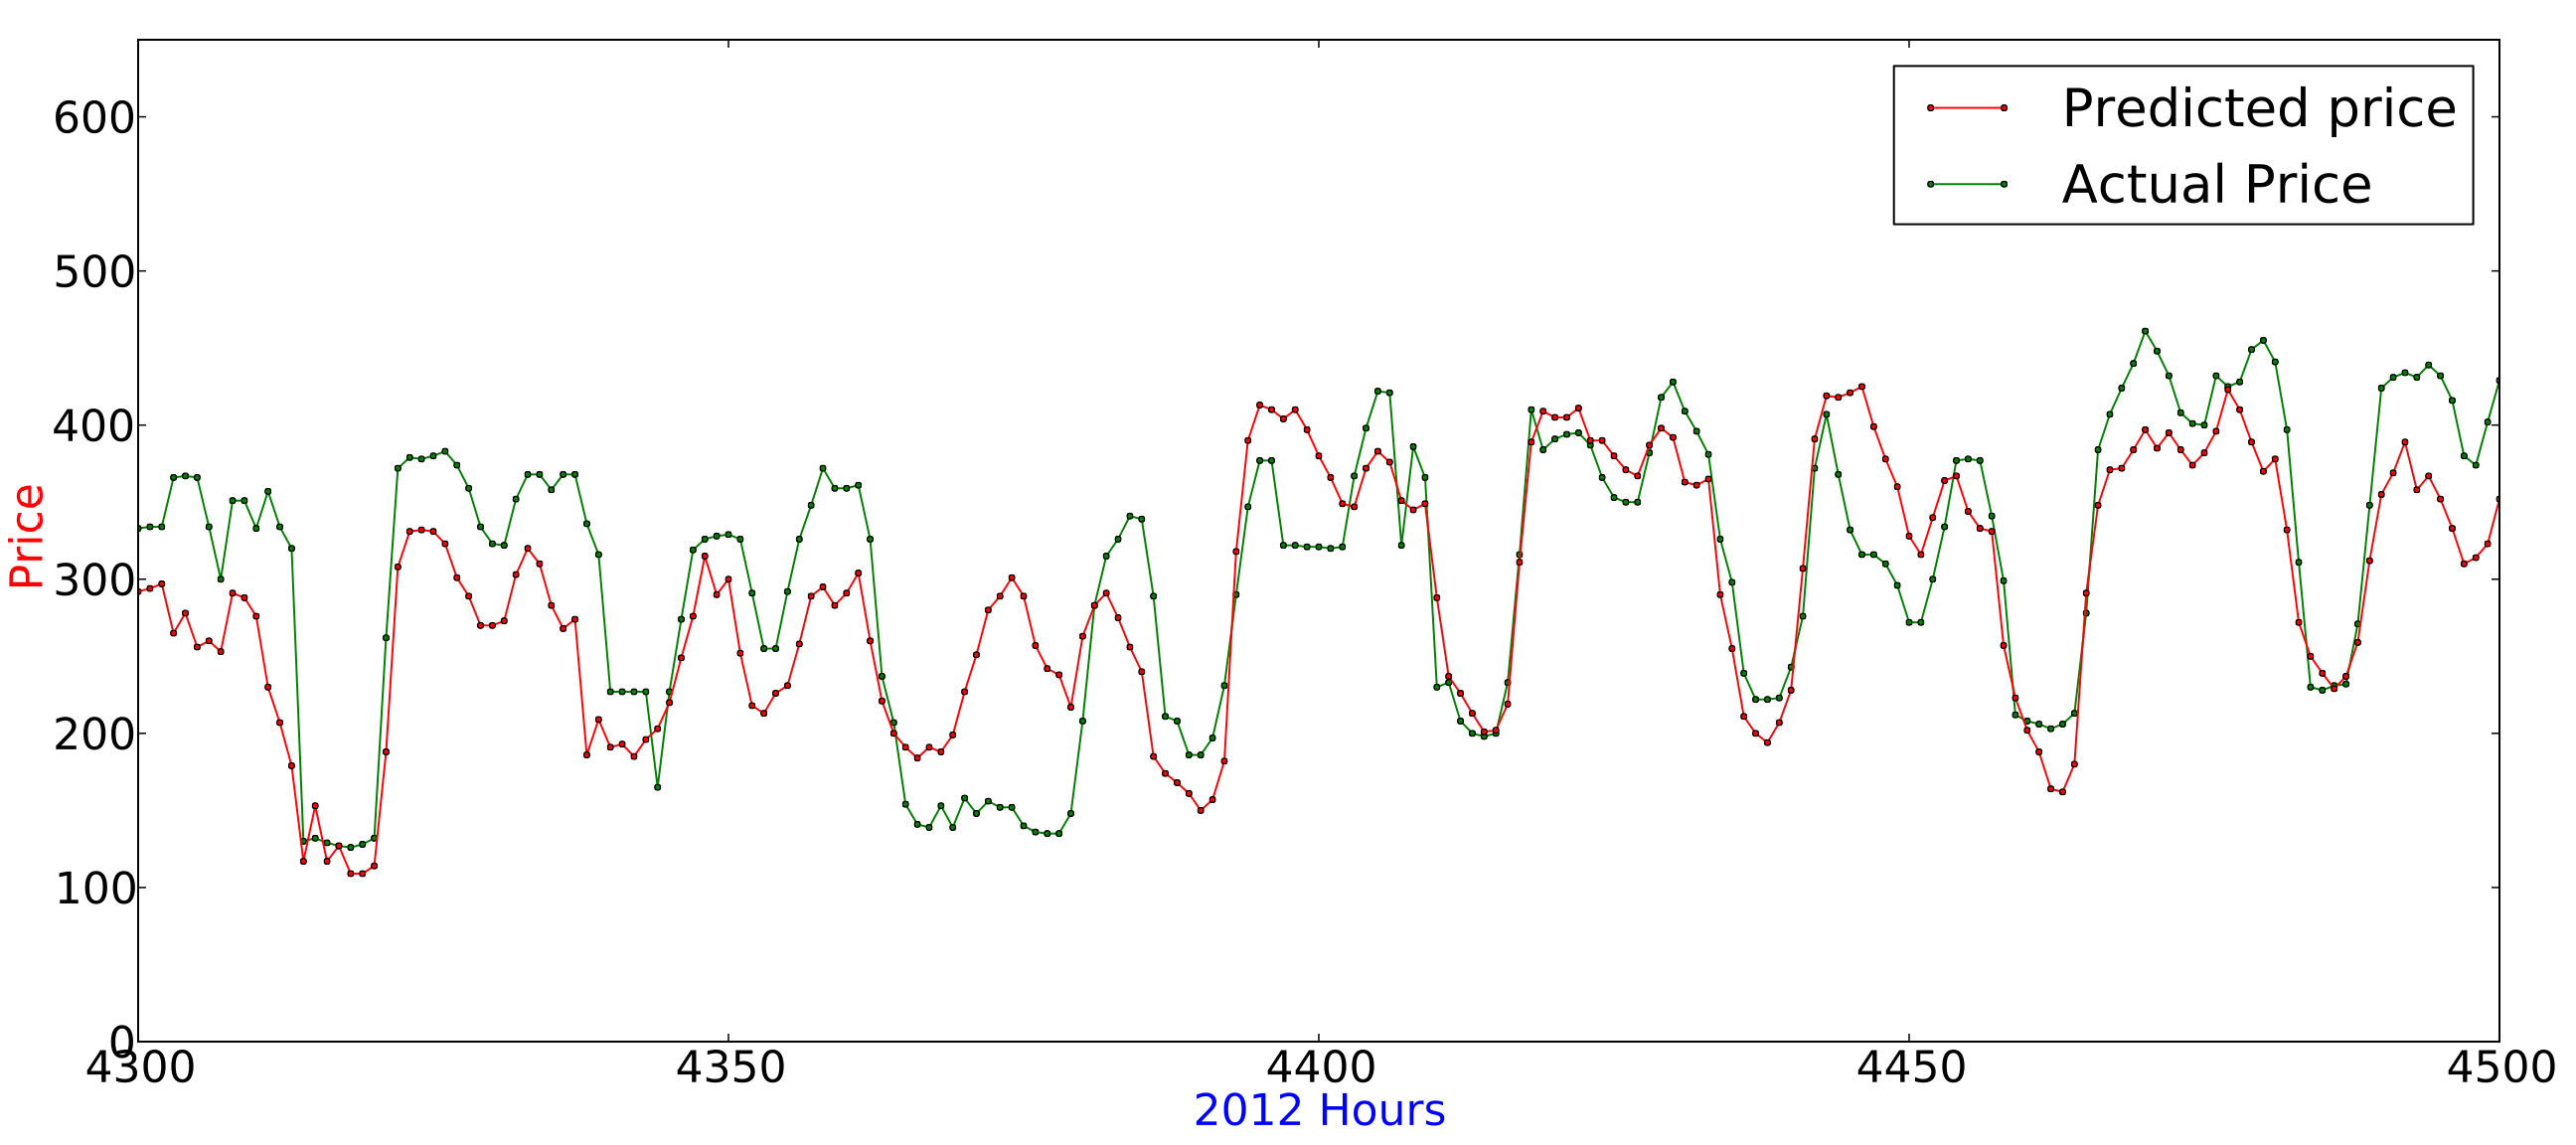
\includegraphics[width=\linewidth]{billeder/PriceExperimentalAnalysis/summer.jpg}
\caption{Electricity price on 200 hours from summer}
\label{fig:abilityToPredictElectricityPrice}
\end{figure}

We have attempted to simulate real use in our experiments by predicting day-ahead prices and wind power productions over a whole year with different offsets where every predicted hour uses the last predicted hour (except from the first hour) which indicates that our modelled ANN can be used in practice. The preconditions for using ANN in practice has been discussed in Section~\ref{} and ..... todo{....}
 
\subsubsection{Concluding Remarks on Feasibility}
The above discussions comply well with the fact that machine learning is not all technical bot also intuition, creativity and black art\cite{18}. For instance a great deal of intuition and creativity goes into designing the experiments. Everything cannot be tested and you must rely on intuition to include all situations necessary for testing, and the creativity resides in how to actually do it. Furthermore, the different inputs can be represented in various ways that calls for creativity --- represent input as a matrix, calculate slope or volatility and represent the seasonal aspect as month or summer/winter/spring/fall. The ANN being black art or a black box requires intuition in itself since we cannot foresee the outcome. When analysing prediction results from the experiments we rely on the analysis but also our intuition, especially in cases where things are not as we expected. We must assume based on the analysis and our intuition that this was what happened. It is again an argument for analysis and experiments to be documented for both own benefit and the sake of transparency for others. The following points sum up the above discussions regarding feasibility of the Artificial Neural Network.

\begin{itemize}
\item We have analysed the influential factors of wind power and electricity prices in western Denmark and verified the best combination through experiments. It has been shown that the feasibility of predictions that originate from an ANN is highly connected to performing a proper analysis and testing it. Furthermore, the need for transparency was highlighted in this context to ensure both trust but also for others to see feasibility in the predictions that use ANN as technology.
\item Strategies have been applied in an attempt to improve accuracy (data manipulation, matrix, black box). We have shown how they can be applied to the inputs and has shown an improvement in accuracy throughout the experiments. The ANN for prediction can be significantly improved by manipulating the dataset to fit the problem and increase its potential accuracy.
\item The experiments must be performed on a satisfying number of days on an unseen testing set. We suggest a year so that most cases are covered in order for the ANN to show its potential in a realistic setup --- this setup convey the potential for practical use due the simulation of many different scenarios during the year. 
\end{itemize}

\todo{the point is that many of the points we are dealing with when modelling the network is directly transferable to the DSS. It puts extra emphasize on why this should be made properly in the first place.}